% 定义文档类型:中文文章
\documentclass{ctexart}

% 导入宏包
\usepackage{tikz}
\usepackage{pgfplots}
\usepackage{geometry}
\usepackage{hyperref}
\usepackage{amsmath}

% 一些包有多个模块,加载指定模块
\usetikzlibrary{positioning}

% 设置超链接样式
\hypersetup{
	colorlinks=true,
	linkcolor=blue,
	filecolor=blue,
	urlcolor=blue,
	citecolor=cyan,
}

% 设置纸张为 A4,版心占页面长度的比例为80%
\geometry{a4paper, scale=0.8}

% 文档标题
\title{人工智能-基础篇}
\author{aszswaz}
\date{2022-03-17}

\begin{document}
\maketitle

\section{Rosenblatt 感知器}
\subsection{最基本的 Rosenblatt 感知器}
Rosenblatt 感知器是第一个从算法上完整描述的神经网络,它向人们展示了计算机对函数的自适应调整的可能性。

假设 $w$ 为斜率、$t$ 为标准答案、$e$ 为误差、$a$ 为学习率($0 \le a \le 1$),感知器的流程图如下:

% 绘制 Rosenblatt 流程图
\begin{center}
	\begin{tikzpicture}[
			% 有圆角的长方形
			squarednode/.style={rectangle, draw=black, minimum size=5mm, rounded corners},
			% 看不见的像素点,用来连接线,达到折线的效果
			point/.style={coordinate, on grid}
		]
		\node[squarednode]      (maintopic)                                                 {输入$x$};
		\node[squarednode]      (gety)          [below of=maintopic]                        {$y = w \cdot x$};
		\node[squarednode]      (error)         [below of=gety]                             {$t - y = e$};
		%Nodes
		\node[squarednode]      (neww)          [below of=error]                            {$n = w + a \cdot e \cdot x$};
		\node[squarednode]      (assgin)        [below of=neww]                             {$w = n$};
		\node[point]            (point1)        [left of=assgin, node distance=2cm]         {point1};

		%Lines
		\draw[->] (maintopic)       --            (gety);
		\draw[->] (gety)            --            (error);
		\draw[->] (error)           --            (neww);
		\draw[->] (neww)            --            (assgin);
		% 绘画一个点,并链接两条线,形成一个折线
		\draw[-]  (assgin)          --            (point1);
		\draw[->] (point1)          |-            (gety);
	\end{tikzpicture}
\end{center}
\url{rosenblatt.py}

Rosenblatt 感知器中,误差 $e$ 的计算公式为 $e = x^2w^2 + (-2xy) + y^2$,在坐标系中,它是一个开口向上的抛物线:$y = ax^2 + bx + c$。

假设坐标系中,存在一个点:$x = 0.4, y = 0.68$,预测误差 $e$ 与斜率 $w$ 的关系为:

$$
	\begin{aligned}
		e & = 0.16w^2 - 0.544 + 1.36 \\
		  & = 0.16w^2 + 0.816
	\end{aligned}
$$

\begin{center}
	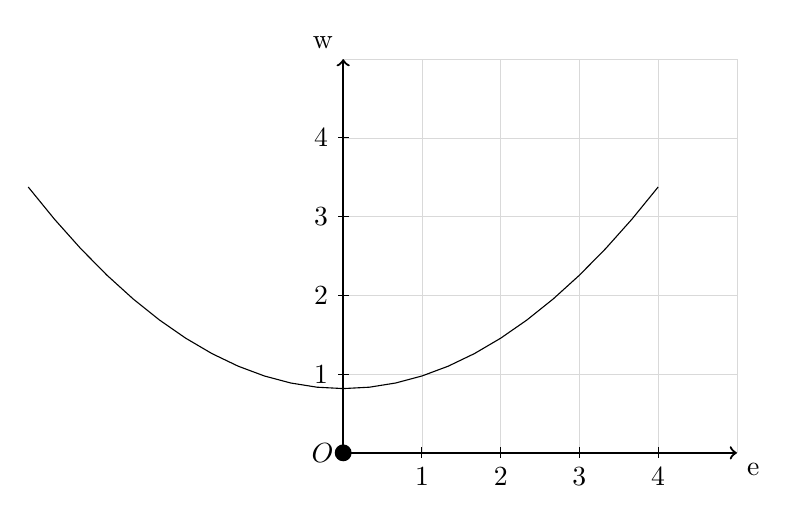
\begin{tikzpicture}
		% 绘制一个大小为 5 * 5 网格线
		\draw[help lines, color=gray!30] (0, 0) grid (5,5);
		% 坐标轴原点
		\draw[fill] (0, 0) node [left]{$O$} circle(.1);
		% 绘制 y 轴和 x 轴
		\draw[thick, ->] (0, 0) -- (5, 0) node[anchor = north west] {e};
		\draw[thick, ->] (0, 0) -- (0, 5) node[anchor = south east] {w};
		% 画 X 轴和 y 轴的刻度
		\foreach \v in {1, ..., 4} {
				% 这里是用一个短短的直线表示刻度的点
				\draw (\v cm, 2pt) -- (\v cm, -2pt) node[anchor = north] {$\v$};
				\draw (2pt, \v cm) -- (-2pt, \v cm) node[anchor = east] {$\v$};
			}
		% 绘制函数在坐标轴上的抛物线
        \draw[domain = -4 : 4] plot (\x, {0.16 * \x * \x + 0.816});
	\end{tikzpicture}
\end{center}

\end{document}
